\documentclass[zad,zawodnik,utf8]{sinol}

\usepackage{hyphenat}
\usepackage{ulem}

\title{Strzelnica}
\id{str}
\RAM{64}
\date{2019-03-02}
\konkurs{PreMOI}

\signature{Kubin}
\author{Jakub Bachurski}

\begin{document}

\begin{tasktext}

\par Kernel poszedł z kolegami na strzelnicę. Aby było zabawnie, uznali, że zliczą, ile razy trafili w cele. Jednak Kernel o tym zapomniał -- na szczęście doskonale pamięta, jakie były cele, i jakie strzały wykonał (ma niewyobrażalnie dobrą pamięć). Niestety, strzelnica była bardzo duża i byli tam bardzo długo, więc nie poradzi sobie samodzielnie wykonać zadania. Czy pomożesz mu zliczyć ile razy trafił w cele?

\par Strzelnicę można opisać w kartezjańskim układzie współrzędnych (początek układu jest w $(0, 0)$). Każdy cel jest prostokątem o bokach równoległych do osi układu współrzędnych, więc można go opisać za pomocą jego lewego dolnego oraz prawego górnego rogu. Każdy wykonany strzał musiał być wykonany tak, że tor ruchu pocisku był równoległy do jednej z osi układu. Zatem strzał można opisać jako prostą pionową lub poziomą. Zakładamy, że Kernel był nieskończenie daleko od celów, i zawsze strzelał w ich stronę -- czyli trafił wszystkie cele, które przecina prosta, która opisuje dany strzał. W szczególności, trafienie w krawędź celu także się liczy.

\section{Wejście}

\par Pierwszy wiersz standardowego wyjścia zawiera trzy liczby całkowite $n, k, l$ $(0 \le n, k, l \le 10^5)$, oznaczające odpowiednio liczbę celów, liczbę strzałów pionowych oraz liczbę strzałów poziomych. W każdym z kolejnych $n$ wierszy znajduje się opis celu, składający się z całkowitych liczb $x_1, y_1, x_2, y_2$ $(0 \le x_1, x_2, y_1, y_2 \le 10^9)$, gdzie $(x_1, y_1)$ to lewy dolny, a $(x_2, y_2)$ to prawy górny róg prostokąta. Zachodzi $x_1 < x_2$ oraz $y_1 < y_2$.
\par Następne wiersze opisują wykonane strzały. W $n{+}2$-gim wierszu znajduje się $k$ całkowitych liczb $a_i$ $(0 \le a_i \le 10^9)$, oznaczających, że $i$-ty z pionowych strzałów można opisać prostą pionową przechodzącą przez punkt $(a_i, 0)$. W kolejnym jest $l$ liczb całkowitych $b_j$ $(0 \le b_j \le 10^9)$, oznaczających, że $j$-ty z poziomych strzałów można opisać prostą poziomą przechodzącą przez punkt $(0, b_j)$.
\par Możliwe, że Kernel wiele razy wykonał taki sam strzał. Możliwe jest także, że cele się pokrywają (częściowo lub całkowicie).

\section{Wyjście}

\par Na wyjście wypisz jedną liczbę całkowitą, oznaczającą sumaryczną ilość przecięć celów przez strzały. Jeżeli strzał przeciął wiele celów, to za każdym razem zwiększamy wynik. Cel trafiony wielokrotnie także jest wiele razy liczony do wyniku (jednak jeden strzał trafia dany cel dokładnie raz).

\pagebreak

\section{Przykłady}
\makeexamplef{in/0.in}{out/0.out}
\subsection{Wyjaśnienie przykładu}
\par Drugi strzał poziomy oraz pierwszy (i jedyny) pionowy przecinają po jednym celu. Za drugim strzałem poziomym Kernel spudłował. Przykład tak wygląda na rysunku:
\par \centering {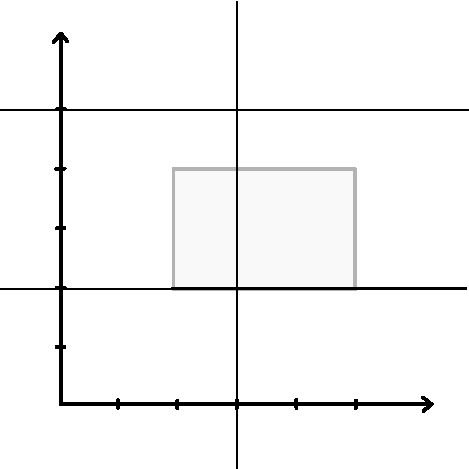
\includegraphics{rys}}

\begin{points}
	\makesubtask{1}{$n, k, l \le 10^3$, współrzędne $x, y \le 10^3$}{10}
	\makesubtask{2}{$n, k, l \le 10^3$}{10}
	\makesubtask{3}{współrzędne $x, y \le 10^5$}{30}
	\makesubtask{4}{brak dodatkowych ograniczeń}{50}
\end{points}

\end{tasktext}
	
\end{document}